\documentclass[aspectratio=1610]{beamer}
%%%%%%%%%%%%%%%%%%%%%%%%%%%%%%%%%%%%%%% Theming
\usetheme[progressbar=frametitle,numbering=fraction]{metropolis}
\addtobeamertemplate{frametitle}{}{%
\begin{textblock*}{100mm}(.85\textwidth,-1cm)
\includegraphics[width=.65cm,trim={0 1.5cm 1.5cm 0}]{figures/UU_logo_vit.pdf}
\end{textblock*}}

\definecolor{black_}{RGB}{25, 25, 25}
\definecolor{blue_}{RGB}{46,131,191}
\definecolor{green_}{RGB}{46,191,106}
\definecolor{uured}{RGB}{191,45,56}
\definecolor{uudarkgrey}{RGB}{130,130,130}
\definecolor{uumidgrey}{RGB}{190,190,190}
\definecolor{uulightgrey}{RGB}{230,230,230}
\setbeamercolor{alerted text}{fg=uured}
\setbeamercolor{example text}{fg=green_}
\metroset{block=fill}
\usepackage{pgfplots}
\pgfplotscreateplotcyclelist{myColorList}{%
        color=blue_,every mark/.append style={fill=blue_},mark=*\\%
        color=uured,every mark/.append style={fill=uured},mark=square*\\%
        color=green_,every mark/.append style={fill=green_},mark=otimes*\\%
        color=black_,every mark/.append style={fill=black_},mark=diamond*\\%
    }
\pgfplotsset{every axis/.append style={cycle list name=myColorList}}


%%%%%%%%%%%%%%%%%%%%%%%%%%%%%%%%%%%%%%%%


\usepackage[most]{tcolorbox}
\usepackage{subcaption}
\usepackage{tikz}
\usetikzlibrary{arrows}
\usetikzlibrary{positioning}
\usetikzlibrary{calc}
\usetikzlibrary{intersections}
\usepackage{pgfplots}	
\pgfplotsset{compat=1.17}
\usepackage{textpos}
\usepackage{amssymb}
\usepackage{amsthm}
\usepackage{mathtools}
\usepackage{booktabs}

% https://tex.stackexchange.com/questions/146908/beamer-overlay-specifications-for-a-tikzpicture
\tikzset{
    invisible/.style={opacity=0,text opacity=0},
    visible on/.style={alt={#1{}{invisible}}},
    alt/.code args={<#1>#2#3}{%
      \alt<#1>{\pgfkeysalso{#2}}{\pgfkeysalso{#3}} % \pgfkeysalso doesn't change the path
    },
  }


\usepackage{biblatex}
\addbibresource{hult_502.bib}

\let\definition\relax

% Qutie general things (not math)
\newcommand\red[1]{\textcolor{red}{#1}}

% Qutie general things (math)
\newcommand{\R}{\mathbb R}

%linalg
\newcommand{\kroneckerDelta}{\delta}
\DeclarePairedDelimiter\norm{\lVert}{\rVert}
\DeclareMathOperator*{\vecop}{vec}
\DeclareMathOperator*{\diag}{diag}
\DeclareMathOperator*{\matop}{mat}
\newcommand{\eye}{I}
\DeclareMathOperator*{\tr}{tr}
\newcommand{\hadamard}{\circ}
\newcommand{\kronecker}{\otimes}
\newcommand{\T}{\top}
\newcommand{\vecOne}{\mathbf{1}}

% stats and probability
\DeclareMathOperator*{\cov}{Cov}
\DeclareMathOperator*{\argmin}{arg\,min}
\newcommand{\convp}{\overset{p}{\to}}
\newcommand{\convd}{\overset{d}{\to}}
\newcommand{\E}{\mathbb{E}}
\newcommand{\En}{\mathbb{E}_n}
\newcommand{\Eint}{\widetilde{\mathbb{E}}}
\newcommand{\covint}{\widetilde{\text{Cov}}}
\newcommand{\varint}{\widetilde{\text{Var}}}
\newcommand{\var}{\text{Var}}
\newcommand{\Prob}{\mathbb{P}}
\newcommand{\normal}{\mathcal N}
\newcommand{\permMat}{\mathcal P}
\newcommand{\unitBasisMatrix}{E}


%% Document variables with semantic meaning in this article
\newcommand{\semCoeffMat}{W}
\newcommand{\semCoeffColumn}{w}
\newcommand{\semCoeffMatSet}{\mathcal W}
\newcommand{\semCoeffOpt}{\semCoeffMat_\circ}

\newcommand{\semCoeffEstN}{\semCoeffMat_\nData}
\newcommand{\dagPermutationMatrix}{P}
\newcommand{\semScaleMatrix}{M}
\newcommand{\semVector}{v}
\newcommand{\semVectorOrdered}{\omega}
\newcommand{\semPermutationMatrix}{P}
\newcommand{\semApproximatorFunction}{f}
\newcommand{\semNoise}{e}
\newcommand{\semNoiseCovariance}{\Sigma}
\newcommand{\semInterventionNoise}{\widetilde \semNoise}
\newcommand{\semInterventionNoiseCovariance}{\widetilde \semNoiseCovariance}
\newcommand{\mutilatingMatrix}{Z}
\newcommand{\cofactorMatrix}{C}
\newcommand{\dNodes}{d}
\newcommand{\linearPredictor}{\mathcal L}
\newcommand{\minorMatrix}{m}
\newcommand{\averageCausalEffect}{\gamma}
\newcommand{\averageCausalEffectTarget}{\averageCausalEffect_\circ}
\newcommand{\averageCausalEffectSet}{\Gamma}
\newcommand{\averageCausalEffectEstN}{\averageCausalEffect_\nData}
\newcommand{\averageCausalEffectNumeric}{\hat{\averageCausalEffectTarget}}
\newcommand{\observationalDistribution}{p}
\newcommand{\interventionalDistribution}{\tilde p}
\newcommand{\lossFunc}{\ell}
\newcommand{\outcomeVar}{y}
\newcommand{\decisionVar}{x}
\newcommand{\adjustmentVar}{z}
\newcommand{\adjusted}[1]{\bar{#1}}
\newcommand{\validAdjustmentVar}{\adjusted{z}}
\newcommand{\decisionOptimal}{\hat \decisionVar }
\newcommand{\decisionTrueOptimal}{\decisionVar ^\star}
\newcommand{\decisionSpace}{ \mathcal X}
\newcommand{\dataSet}{\mathcal D}
\newcommand{\nData}{n}
\newcommand{\dagTolerance}{\epsilon}
\newcommand{\dagToleranceMax}{\dagTolerance_\star}
\newcommand{\mEstParameter}{\theta}
\newcommand{\mEstParameterEstN}{\mEstParameter_\nData}
\newcommand{\mEstParameterTrue}{\mEstParameter_\circ}
\newcommand{\mEstParameterSet}{\Theta}
\newcommand{\mEstParametrization}{L}
\newcommand{\mEstLoss}{\ell}
\newcommand{\mEstConstrint}{g}
\newcommand{\mEstCovarianceN}{\mathcal J_\nData}
\newcommand{\regCoefficient}{\beta}
\newcommand{\regCoefficientSet}{B}
\newcommand{\eps}{\varepsilon}
\newcommand{\confidenceLevel}{\alpha}
\newcommand{\hFun}{h}
\newcommand{\qMatrix}{\mathsf{Q}}

% helpers for m-estimation proof
\newcommand{\Un}{U_n}
\newcommand{\Qn}{Q_n}
\newcommand{\Qtrue}{Q_\circ}
\newcommand{\Utrue}{U_\circ}
\newcommand{\Jn}{J_n}
\newcommand{\Kn}{K_n}
\newcommand{\Ktrue}{K_\circ}
\newcommand{\Jtrue}{J_\circ}
\newcommand{\nablatheta}{\nabla}
\newcommand{\PiTrue}{\Pi_\circ}
\newcommand{\PiN}{\Pi_n}

% helpers for augmented lagrangian method
\newcommand{\augLagSlack}{s}
\newcommand{\augLag}{\mathcal L}
\newcommand{\augLagLagMul}{\alpha}
\newcommand{\augLagPen}{\rho}
\newcommand{\augLagPenMul}{\mu}
\newcommand{\augLagPenMax}{\augLagPen_{max}}
\newcommand{\augLagIter}{k}
\newcommand{\augLagMinImprovement}{g}
\newcommand{\augLagContraint}{c}
\newcommand{\augLagConstraintTol}{\eta}

% helpers for discussin misspacified error covariance
\newcommand{\assStruct}{\widehat{\semNoiseCovariance}} % assumed latent covariance structure
\newcommand{\semNoiseScale}{s}
\newcommand{\misspecCond}{\kappa\left(\assStruct^{-1}\semNoiseCovariance\right)}

%repeated acroynoms
\newcommand{\DAG}{\textsc{dag}}
\newcommand{\scm}{\textsc{scm}}
\newcommand{\OLS}{\textsc{ols}}

\newcommand{\blueGamma}{\textcolor{blue_}{\averageCausalEffectSet_{\confidenceLevel, \nData}}}

\title{Inference of Causal Effect when Control Variables are Unknown}
\author{Ludvig Hult and Dave Zachariah}
%\institute{37th Conference on Uncertainty in Artificial Intelligence}
\institute{Department of Information Technology, Uppsala University, Sweden}
\date{2021}
\titlegraphic{\flushright\includegraphics[width=.1\textwidth]{figures/UU_logo.pdf}}

\begin{document}

\frame{\titlepage}

%
% MOTIVATION
%
\section{Intro}
\begin{frame}{Example: Observational Study (inspired by \cite{luoca_2021})}
    \centering
    \begin{tikzpicture}[
      ->,>=stealth',
      shorten >=1pt,
      auto,
      semithick,
      every node/.append style={color=black_},
      every path/.append style={color=uumidgrey},
      ]
      \node[circle,draw, minimum size=20pt,font=\tiny] (Z2) at (2,2) { BMI};
      \node[circle,draw, minimum size=20pt,color=green_] (X) at (-2,0) {\includegraphics[width=1cm]{figures/vitamin-icon-21420.png}};
      \node[circle,draw, minimum size=20pt,color=uured] (Y) at (2,0) {\includegraphics[width=1cm]{figures/toppng.com-coronavirus-covid-19-icon-512x512.png}};
      \node[circle,draw, minimum size=20pt] (Z1) at (-2,-2) {...};
      \node[circle,draw, minimum size=20pt,font=\tiny,align=left] (BP) at (4,2) { Blood \\  Pressure};
      \node[circle,draw, minimum size=20pt,font=\tiny,align=left] (GENDER) at (-3,3) { Gender };
    
      \path (Z1) edge node[above] {?} (X)
      (Z1) edge node[above] {?}  (Y)
      (X) edge node[above] {?}  (Z2)
      (Z2) edge node[above] {?}  (Z1)
      (X) edge[color=blue_] (Y)
      (Y) edge node[above] {?}  (Z2)
      (Y) edge node[above] {?}  (BP)
      (Z2) edge node[above] {?}  (BP)
      (GENDER) edge node[above] {?}  (X)
      (GENDER) edge node[above] {?}  (Y)
      (GENDER) edge node[above] {?}  (BP);
    \end{tikzpicture} 

\end{frame}
\begin{frame}{Our contribution}
    \centering
    \begin{tcolorbox}[width=10cm]
        We propose a method to get \textbf{valid confidence intervals} for the causal effect parameter when the \textbf{control variabels are unknown}.
    \end{tcolorbox}
\end{frame}

%%%%%%%%%%%%%%%%%%%%%%%%%%%%%%%%%%%%%%%%%%%%

\section{Problem Setup}
\begin{frame}{Interventional data distribution and CEP}
If we intervene on $\decisionVar$ in a system, we observe outcome $\outcomeVar$, they are distributed as the \textbf{interventional distribution}
\[(\decisionVar,\outcomeVar)  \sim \interventionalDistribution(\outcomeVar | \decisionVar) \interventionalDistribution(\decisionVar) \]
\[\Eint[x]=\Eint[y]=0\]
\pause
Can we infer the \textbf{causal effect parameter (CEP)}
\begin{align*}
\averageCausalEffect =   \argmin_{\bar{\averageCausalEffect}} \; \Eint\left[ \big( \Eint[\outcomeVar|\decisionVar]  - \bar{\averageCausalEffect}\decisionVar \big)^2 \right]
\end{align*}
using only observational data?
\end{frame}

\begin{frame}{Observational Data Distribution: Linear Additive Causal model}
    
    \[\semVector = \semCoeffMat^\T\semVector + \semNoise,\]
    \[\E[\semNoise]=0 \quad \var[\semNoise] = \semNoiseCovariance \text{ diagonal and known} \]
    \[v^T{}=(x,y,z_1,z_2,...z_{d-2})^T{}\]
\pause
    where
\begin{itemize}
    \item matrix $\semCoeffMat$ specifies a directed graph $\mathcal G$
    \item we call $\semCoeffMat$ a $\DAG$-matrix if $\mathcal G$ is a acyclic
    \item we consider only DAGs; $W_{i,i}=0 \, \forall i$ is necessary
\end{itemize}
\pause
For this model $\averageCausalEffect(\semCoeffMat)$ has a \textbf{closed form expression}.
\end{frame}

\begin{frame}{$\dagTolerance$-almost DAGs}
From the \emph{DAGs with NO TEARS} paper \cite{zheng_dags_2018}, we know that 
\[ h(W) \coloneqq \tr \exp (\semCoeffMat \hadamard \semCoeffMat)-\dNodes\]
\[ \hFun(\semCoeffMat) =0 \Leftrightarrow \semCoeffMat \text{ is \DAG-matrix}  \]
\pause
We introduce $\dagTolerance$-almost \DAG{}-matrices, defined as
\begin{align*}
\label{eq:def:semCoeffMatSet}
\semCoeffMatSet_\dagTolerance = \left\{ \semCoeffMat\, \middle| \hFun(\semCoeffMat) \leq \dagTolerance  \text{ and } \diag(\semCoeffMat)=0 \right\}
\end{align*}
\end{frame}

\begin{frame}{Target Quantity and Problem Statement}
\begin{columns}
    \begin{column}{0.8\textwidth}
        \begin{equation*}
            \semCoeffOpt \coloneqq \argmin_{\semCoeffMat \in \semCoeffMatSet_\dagTolerance} \; \E\Big[ \norm{\semNoiseCovariance^{-1/2}  \left(\eye - \semCoeffMat^\T \right)\semVector }^2 \Big] 
        \end{equation*}
        \begin{equation*}
            \textcolor{uured}{\averageCausalEffectTarget} = \averageCausalEffect(\semCoeffOpt)
        \end{equation*} 
        \uncover<2->{
        \begin{block}{Problem Statement}
            Construct a confidence interval $\blueGamma$
            for \textcolor{uured}{$\averageCausalEffectTarget$}, that covers with probability $1-\confidenceLevel$, using $\nData$ data points?
        \end{block}
        }
    \end{column}
    \begin{column}{0.2\textwidth}
        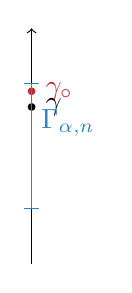
\begin{tikzpicture}
            \draw[->] (0,0) -- (0,3);
            \node at (0,2) [circle,fill=black,label=right:$\averageCausalEffect$,inner sep=1pt] {};
            \node[text=uured] at (0,2.2) [circle,fill=uured,label=right:{\textcolor{uured}{$\averageCausalEffectTarget$}},inner sep=1pt] {};
            \draw[|-|,color=blue_,visible on=<2->]
                (0,0.7) 
                -- node[anchor=south west]{$\averageCausalEffectSet_{\confidenceLevel,\nData}$}
                +(0,1.6);
        \end{tikzpicture}
    \end{column}
    \end{columns}
\uncover<3->{
Assuming unicity of $\semCoeffOpt$. For $\dagTolerance=0$, there is a unique solution, by \cite{loh_high-dimensional_2014}. For $\dagTolerance>0$ it is an open problem.
}
\end{frame}




\section{Results}

\begin{frame}{CI Formulation}
\begin{theorem}[Theorem 4]
    There is a CI $\blueGamma$ with coverage
    \begin{equation*}
    \lim_{\nData \rightarrow \infty} \: \Prob ( \averageCausalEffectTarget \in  \blueGamma  ) = 1 - \alpha,
    \end{equation*}
        given by
            \begin{align*}
            \blueGamma  = \left\{ \averageCausalEffect \in \R \middle|\frac{1}{\nData} \frac{ (\averageCausalEffect - \averageCausalEffect(\semCoeffEstN))^2}
            {  \nabla \averageCausalEffect(\semCoeffEstN)^\T\mEstCovarianceN \nabla \averageCausalEffect(\semCoeffEstN)}  \leq \chi^2_{1,\confidenceLevel}  \right\}
        \end{align*}
        has asymptotic coverage probability
    where $\chi^2_{1,\confidenceLevel}$ denotes the $(1-\alpha)$ quantile of the chi-squared distribution with 1 degree of freedom, and 
    $\mEstCovarianceN$ is a Fisher information, projected onto the constraint set.
    \label{thm:confidence_set_for_ace}
    \end{theorem}
    \note{Wald kind of statistic}
\end{frame}


\begin{frame}{CI by Projection: 2D Case}

    \begin{figure}
        \pgfkeyssetvalue{/figure/width}{10cm}
        \pgfkeyssetvalue{/figure/height}{5cm}
        \pgfmathsetlengthmacro\sideWidth{3cm}
\pgfmathsetlengthmacro\axisHeight{\pgfkeysvalueof{/figure/height}}
\pgfmathsetlengthmacro\axisWidth{\pgfkeysvalueof{/figure/width}-\sideWidth}
\begin{tikzpicture}
\begin{axis}[
    axis lines = left,
    height=\axisHeight,
    width=\axisWidth,
    xlabel = $\semCoeffMat_{2,1}$,
    ylabel = $\semCoeffMat_{1,2}$
    ,xmin=-.1
    ,xmax=2
    ,ymin=-0.1
    ,ymax=2
    ,restrict y to domain=0:2
]
    \coordinate (wTrue) at (axis cs:1,0.5);


    % The unconstrained problem
    \draw[color=green_] (wTrue) ellipse [x radius=1*1.0, y radius=0.5*1.0];
    \draw[color=green_] (wTrue) ellipse [x radius=1*0.8, y radius=0.5*0.8];
    \draw[color=green_] (wTrue) ellipse [x radius=1*0.5, y radius=0.5*0.5];
    \addlegendimage{color=green_}
    \addlegendentry{$\En[\mEstLoss_{\semCoeffMat}(v)]$ level sets}

    \node[label=$\semCoeffMat_\star$,circle,fill,inner sep=2pt] at (wTrue) {};

    % the constraint is in 2D given by 
    % theta1 = +- arccosh[ (epsilon/2)+1 ]/ theta2
    % So in python, the following computes the constant
    % In[1]: import math; eps = 1e-2; math.acosh((1e-2/2)+1)
    % Out[1]: 0.09995838013869626
    \addplot [
        domain=0.000001:4, 
        samples=400, 
        color=black_,
        name path global=hFunLine,
        visible on=<2->
        ]
        {0.099/x};
    \addlegendentry{$\hFun(\semCoeffMat)-\dagTolerance=0$}

    \path[name path=axhline] (wTrue) -- +(0,-10cm);
    \fill[uured,name intersections={of=axhline and hFunLine},visible on=<2->]
        (intersection-1) circle(1mm) node[above left] {$\semCoeffEstN$};

    % The tangent line is hand drawn on top
    \draw[|-|,blue_,very thick,visible on=<3>] (axis cs:0.7,0.14) -- (axis cs:1.4,0.06);
    %\addlegendimage{blue_, very thick}
    %\addlegendentry{Confidence set for $\semCoeffEstN$}

\end{axis}
\coordinate (gammaLineBottom) at (\axisWidth,-1cm);
\coordinate (gammaEstN) at ($(gammaLineBottom)+(0,\axisHeight/2)$);
\draw[->] (gammaLineBottom) -- ++(0,\axisHeight);
\fill[uured,visible on=<2->]
      (gammaEstN)
      circle(1mm) 
      node[right] {$\averageCausalEffect(\semCoeffEstN)$};
\draw[|-|,color=blue_,visible on=<3>, very thick]
    ($(gammaEstN)-(0,1cm)$)
    -- node[anchor=east]{$\averageCausalEffectSet_{\confidenceLevel,\nData}$}
    ++(0,2cm);
\end{tikzpicture}

        \caption{
            Illustration of Projection Method, when $\dNodes=2$. 
            In that case $\semCoeffMat=\begin{bmatrix}0&\semCoeffMat_{1,2}\\\semCoeffMat_{2,1} & 0 \end{bmatrix}$. When $\dagTolerance \geq \dagToleranceMax$ $\semCoeffEstN = \semCoeffMat_\star$
            }
    \end{figure}
\end{frame}


\begin{frame}{Sanity Checks}
\begin{figure}
    \centering
    \begin{subfigure}[b]{0.45\textwidth}
        \centering
        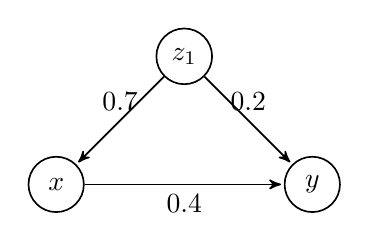
\begin{tikzpicture}[->,>=stealth',shorten >=1pt,auto,node distance=2.3cm,semithick]
  %\tikzstyle{every node}=[fill=none,draw=none]
 % https://tex.stackexchange.com/questions/445946/how-set-tikz-circle-radius-in-nodecircle
  \node[circle,draw, minimum size=20pt] (Z1) {$\adjustmentVar_1$};
  \node[circle,draw, minimum size=20pt] (X) [below left of=Z1] {$\decisionVar$};
  \node[circle,draw, minimum size=20pt] (Y) [below right of=Z1] {$\outcomeVar$};
  

  \path (Z1) edge node[above] {$0.7$} (X);
  \path(Z1) edge node[above] {$0.2$} (Y);
  \path(X) edge node[below] {$0.4$} (Y);
\end{tikzpicture}

        \caption{Underlying causal structure}
        \label{fig:fork_dag}
    \end{subfigure}
    \hfill
    \begin{subfigure}[b]{0.45\textwidth}
        \centering
        \input{tikz/3node_fork_chart.tikz}
        \caption{$95\%$-confidence intervals that aim to cover $\averageCausalEffectTarget$. $\blueGamma$ is CI for our method. $\regCoefficientSet_{\confidenceLevel,\nData}$ is HC0 CI for OLS.}
        \label{fig:fork_asymptotics}
    \end{subfigure}
    \hfill
\end{figure}
\end{frame}


\begin{frame}{Sanity Checks}
\begin{figure}
    \centering
    \begin{subfigure}[b]{0.45\textwidth}
        \centering
        \tikzset{node distance=2.3cm}
        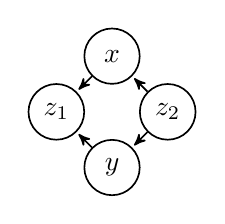
\begin{tikzpicture}[->,>=stealth',shorten >=1pt,auto,semithick]
  %\tikzstyle{every node}=[fill=none,draw=none]
 % https://tex.stackexchange.com/questions/445946/how-set-tikz-circle-radius-in-nodecircle
  \node[circle,draw, minimum size=20pt] (Z2) {$\adjustmentVar_1$};
  \node[circle,draw, minimum size=20pt] (X) [above right of=Z2] {$\decisionVar$};
  \node[circle,draw, minimum size=20pt] (Y) [below right of=Z2] {$\outcomeVar$};
  \node[circle,draw, minimum size=20pt] (Z1) [below right of=X] {$\adjustmentVar_2$};

  \path (Z1) edge  (X)
  (Z1) edge   (Y)
  (X) edge   (Z2)
  (Y) edge   (Z2);
\end{tikzpicture}

        \caption{Underlying causal structure. All edges has value 1.}
        \label{fig:collider_dag}
    \end{subfigure}
    \hfill
    \begin{subfigure}[b]{0.45\textwidth}
        \centering
        \pgfplotsset{every axis/.append style={width=\columnwidth, height=.6\columnwidth}}
        \begin{tikzpicture}[baseline]
    \pgfplotstableread[col sep=comma]{./data/4node_collider_summary.csv}{\datatable};
    \begin{semilogxaxis}[
        xlabel={No. of data points, $\nData$},
        ylabel={Parameter $\averageCausalEffect$},
        xmin=90,
        xmax=11000,
        legend style={
            font=\scriptsize, at={(0.5,1.10)},
            anchor=south,legend columns=-1},
    ]
        \addplot+ [ only marks, mark=*, mark size=1pt,
            error bars/.cd,
            y dir=both,
            y explicit] table [x=m_obs, y=ace_value, y error=q_ace_standard_error] {\datatable};
        \addplot+ [only marks, mark=*, mark size= 1 pt,
            error bars/.cd,
            y dir=both,
            y explicit] table [x=m_obs, y=ols_value, y error=q_ols_standard_error] {\datatable};
        \addplot [no markers] table [x=m_obs, y=ace_circ] {\datatable};
        \legend{{$\averageCausalEffectSet_{\confidenceLevel,\nData}$},{$\regCoefficientSet_{\confidenceLevel,\nData}$},{$\averageCausalEffectTarget$}}
    \end{semilogxaxis}
\end{tikzpicture}

        \caption{$95\%$-confidence intervals that aim to cover $\averageCausalEffectTarget$.
        $\blueGamma$ is CI for our method. $\regCoefficientSet_{\confidenceLevel,\nData}$ is HC0 CI for OLS.}
        \label{fig:collider_asymptotics}
    \end{subfigure}
    \hfill
\end{figure}
\end{frame}


\begin{frame}{Compare with LiNGAM\cite{shimizu_directlingam_2011, hyvarinen_pairwise_2013}}
\begin{table}
    \centering
    \caption{Empirical coverage rate (CR) and the average Confidence Interval (CI) width for LiNGAM Bootstrap CI and $\averageCausalEffectSet_{\confidenceLevel,\nData}$ proposed in this article. The nominal CR was set to exceed $1-\alpha = 95\%$.}\label{tab:lingam_compare}
    \begin{tabular}{lllrr}
       \toprule
       Noise  & Method & CR    & Avg CI width & Avg $\averageCausalEffectEstN$ \\
       \midrule
       Normal & LiNGAM & 100\% & 2.01         & 0.64                           \\
              & our    & 99\%  & 0.15         & 1.79                           \\
       Exp    & LiNGAM & 92\%  & 0.08         & 1.77                           \\
              & our    & 100\% & 0.54         & 1.79                           \\
       Gumbel & LiNGAM & 85\%  & 0.07         & 1.77                           \\
              & our    & 100\% & 0.46         & 1.79                           \\
       \bottomrule
\end{tabular}

\end{table}
\end{frame}

\section{Conclusions}

\begin{frame}{Conclusions}
    \begin{itemize}[<+->]
        \item We derive \textbf{valid confidence interval} under \textbf{unknown control variables}
        \item Assumptions rests on \textbf{no hidden confounding} -- known diagonal latent covariance
        \item Constrained risk minimization asymptotics derived by \textbf{projection technique}
        \item Numerical verifications shows \textbf{valid intervals} where DirectLiNGAM fails
        \item \textbf{Open questions} on identifiability - numerical experiments are promising
    \end{itemize}
\end{frame}

\begin{frame}[allowframebreaks]{References}
    \printbibliography[heading=none]
\end{frame}

\begin{frame}{Contact}
    \textbf{Ludvig Hult, Uppsala University}\\
    \texttt{ludvig.hult@it.uu.se}\\
    \texttt{ludvig.hult@gmail.com}\\
    \url{https://twitter.com/el_hult}\\
    \url{https://github.com/el-hult}
\end{frame}

\end{document}